\documentclass{beamer} 
\usetheme{default} 
\usecolortheme{albatross}
%\setbeamercovered{transparent}
%\useoutertheme{umbcfootline}  


\usepackage[spanish]{babel}
%\usepackage[latin1]{inputenc}
\usepackage[utf8x]{inputenc}
\usepackage{hyperref}
\usepackage{color}
\usepackage{animate}
\usepackage{multicol}
\usepackage{graphicx}
\usepackage{movie15}
\title{Entornos de desarrollo integrados}

\author{Manuel J. Molino Milla \and Luis Molina Garzón}

\date{\today} %

\institute{IES Virgen del Carmen \and Departamento de Informática}




%\beamerdefaultoverlayspecification{<+->}

\begin{document}


\begin{frame}
  \titlepage
\end{frame}

\begin{frame}
    \frametitle{Logo}
\begin{figure}

\includegraphics[scale=1]{imagenes/logo.jpeg} 
\caption{Logo Java}
\end{figure}
\end{frame}

\begin{frame}
  \frametitle{Contenido}
 \tableofcontents[pausesections]
\end{frame}

\section{Eclipse}
\subsection{Introducción}
\begin{frame}
\frametitle{IDE}
\begin{itemize}[<+->]
\item Acrónimo en inglés de integrated development environment
\item Es un programa informático compuesto por un conjunto de herramientas de programación. 
\item Puede dedicarse en exclusiva a un solo lenguaje de programación o bien puede utilizarse para varios.
\item Suele estar compuesto por:
\begin{enumerate}[<+->]
\item Un editor de texto.
\item Un compilador.
\item Un intérprete.
\item Un depurador.
\item Un cliente.
\item Posibilidad de ofrecer un sistema de control de versiones.
\item Factibilidad para ayuda en la construcción de interfaces gráficas de usuario.
\end{enumerate}
\end{itemize}
\end{frame}

\subsection{IDE}
\begin{frame}
\frametitle{IDE}
\begin{Large}
\begin{itemize}[<+->]
\item Eclipse
\item Netbeans
\item IntelliJ IDEA
\item Android Studio
\item JBuilder
\item JDeveloper
\item KDevelop
\item Anjunta
\item MS Visual Studio
\item \dots
\end{itemize}
\end{Large}
\end{frame}

\subsection{Eclipse como IDE}
\begin{frame}
\frametitle{Eclipse}
\begin{itemize}[<+->]
\item Es una plataforma de desarrollo, diseñada para ser extendida de forma indefinida a través de plug-ins.
\item No tiene en mente un lenguaje específico, sino que es un IDE genérico.
\item Goza de mucha popularidad entre la comunidad de desarrolladores del lenguaje Java usando el plug-in JDT que viene incluido en la distribución estándar del IDE.
\item Para lenguaje C y C++, tenemos el plugin CDT.
\item Para pyhton tenemos PyDev
\item Para javascript podríamos usar VJET.
\item \dots
\end{itemize}
\end{frame}

\begin{frame}
\frametitle{Eclipse} 
\begin{figure}
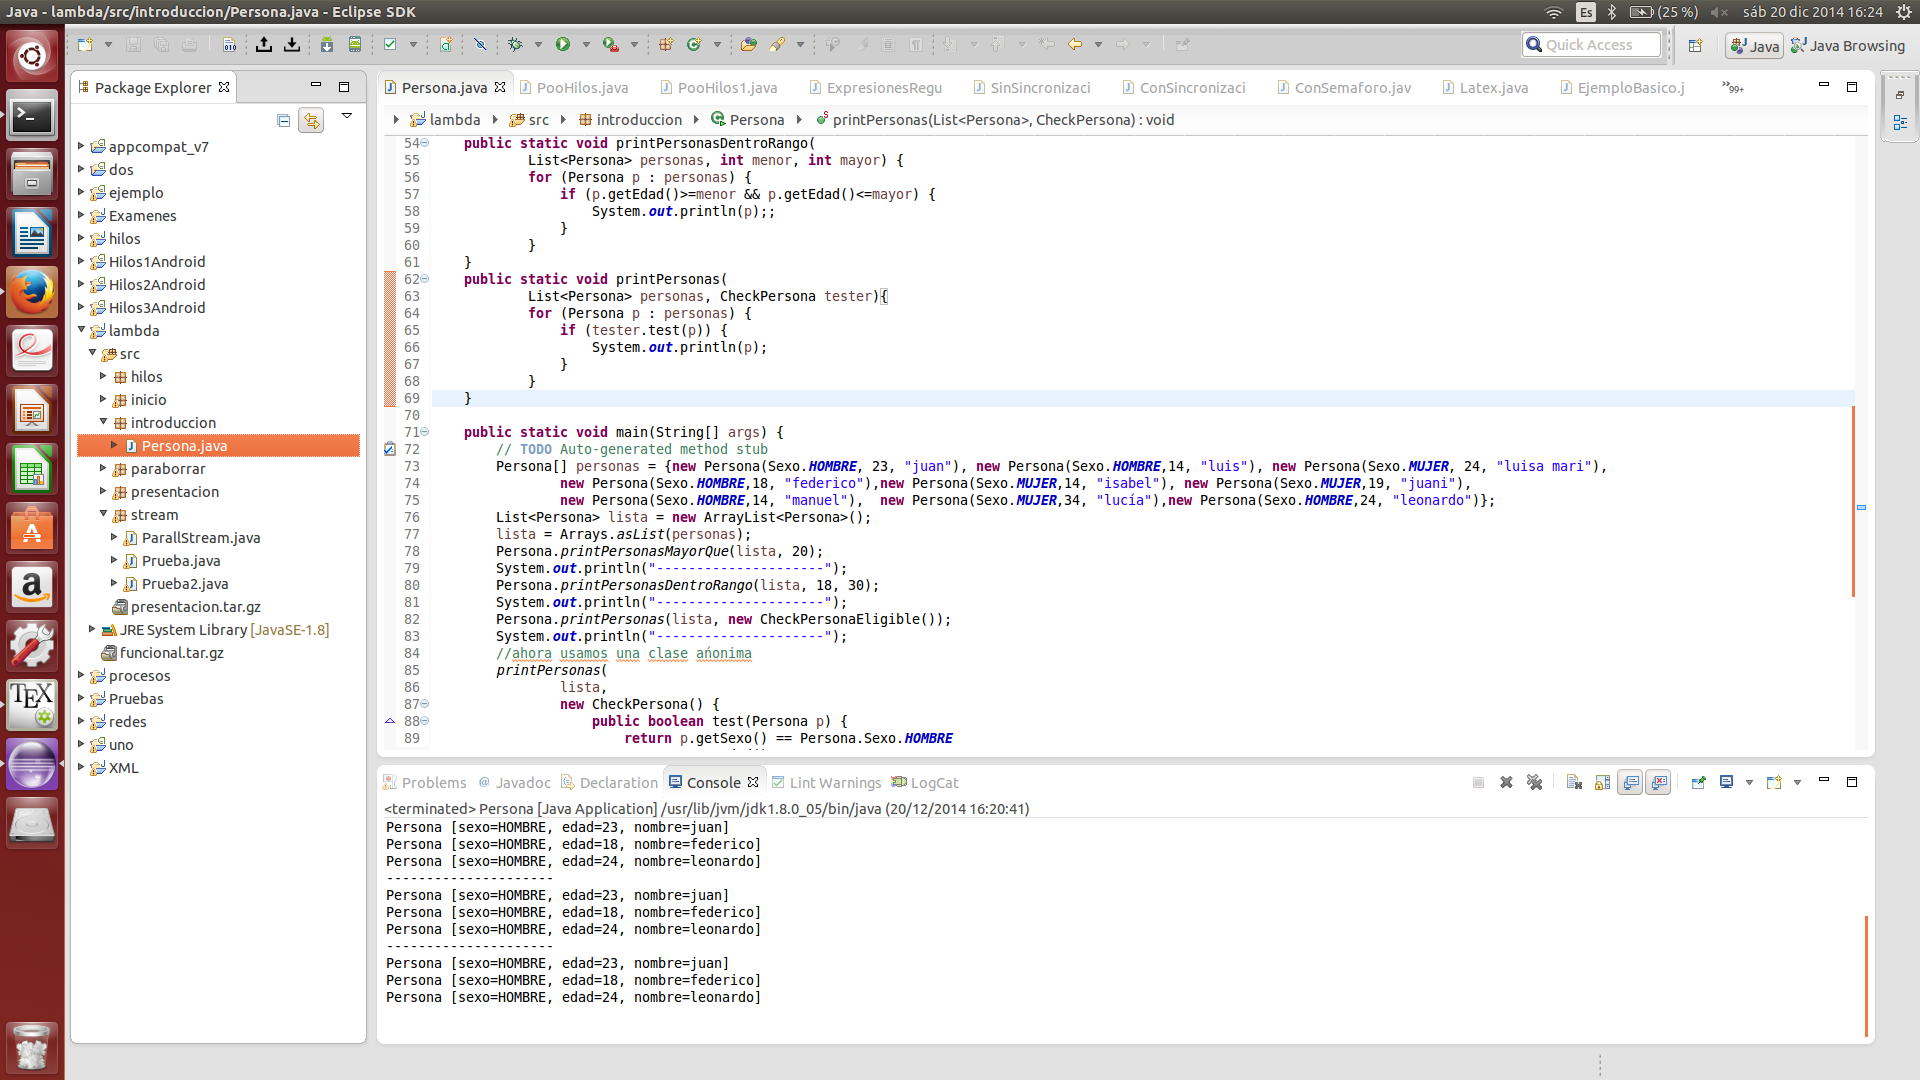
\includegraphics[scale=0.16]{imagenes/eclipse1.png} 
\end{figure} 
\end{frame}

\begin{frame}[fragile]
\frametitle{Ejercicio}
\framesubtitle{Péndulo}
\begin{figure}
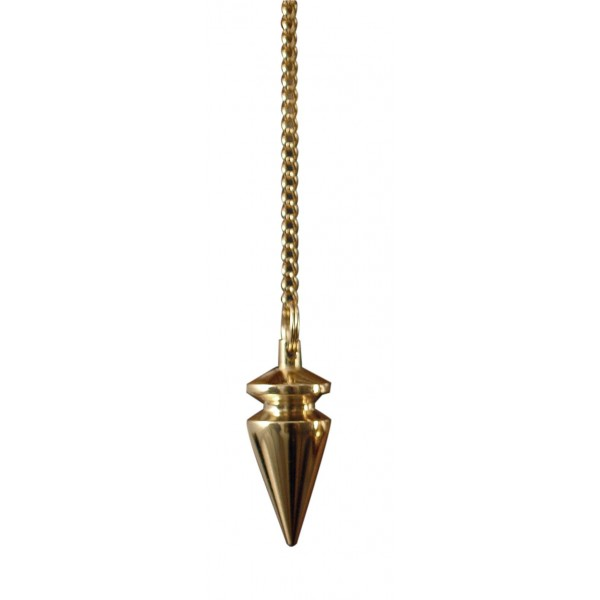
\includegraphics[scale=0.2]{imagenes/pendulo.jpg} 
\end{figure}
\begin{verse}
El periodo de un péndulo es el tiempo que tarde en realizar una oscilación. Se calcula:\\
\begin{center}
$2\pi\sqrt{\frac{l}{g}}$
Donde \emph{l} es la longitud del péndulo y \emph{g} la aceleración de la gravedad.
\end{center}\end{verse}
\end{frame}

\begin{frame}
\frametitle{Péndulo}
Crea un proyecto java denominado \emph{intruducción}, posteriormete incorpora en él un package denominado \emph{pendulo} que tenga en cuenta las dos siguientes clases:\\
Una clase en denominda \emph{Pendulo.java} y una clase \emph{TestPendulo.java}, de acuerdo al siguiente diagrama \emph{UML}:
\begin{figure}
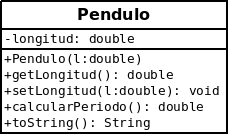
\includegraphics[scale=0.5]{imagenes/Pendulo.png}
\end{figure}
En la clase \emph{TestPendulo.java} debes crear un objeto de tipo \emph{Pendulo} y calcular su periodo de oscilación. Posteriormente cambia el valor de su longitud y volver a calcular el periodo. Para variar el valor de la longitud utiliza la clase \emph{Scanner} y también prueba pasar dicha longitud como argumento. \\ 
Posteriormente crea un \emph{jar ejecutable} y comprueba su funcionamiento.
\end{frame}

\begin{frame}
\frametitle{Ejercicio}
\begin{block}{Librerías externas}
Compila un fichero ejemplo que suministra la documentación del proyecto \emph{itextpdf} que no hayas realizado todavía. Para esto tendrá que incorporar a tu proyecto de eclipse una libreria externa.
\end{block}
\pause
\begin{block}{javadoc}
Crea una clase que represente a un alumno del ciclo formativo. Crea los atributos pertinentes y métodos que creas necesarios. Posteriormente genera la documentación.
\end{block}
\pause
Realiza cada ejercicio en el proyecto que antes has creado, pero cada uno de ellos en \emph{packages} diferentes.
\end{frame}

\subsection{Eclipse y git}
\begin{frame}
\frametitle{Control de versiones}
\begin{itemize}[<+->]
\item Eclipse suele incorpar sistemas de control de versiones tales como CVS y git.
\item En su defecto podemos incorporar un plugin para git, denominado egit.
\item Para su utilización en un proyecto con boton derecho, team y share project
\item A partir de ahí se indica si se quiere usar \emph{CSV} o \textit{git}, y datos como directorio del repositorio local, \dots
\item También tenemos una perpectiva de trabajo en git, donde podemos hacer las operaciones habituales de git: \emph{commit}, \emph{push}, \textit{pull}, \dots
\end{itemize}
\end{frame}

\begin{frame}
\frametitle{Ejercicio}
\begin{verse}
\begin{LARGE}
Sincroniza el proyecto anterior con tu repositorio externo de gitHub.

\end{LARGE}\end{verse}
\end{frame}

\begin{frame}
\frametitle{Preguntas} 
\begin{figure}

\includegraphics[scale=0.9]{imagenes/dudas.png} 
\end{figure} 
\end{frame}

\end{document}

